\documentclass[journal,12pt,twocolumn]{IEEEtran}
\usepackage{setspace}
\usepackage{gensymb}
\usepackage{xcolor}
\usepackage{caption}
\singlespacing
\usepackage{siunitx}
\usepackage[cmex10]{amsmath}
\usepackage{hyperref}
\usepackage{amsthm}
\usepackage{mathrsfs}
\usepackage{txfonts}
\usepackage{stfloats}
\usepackage{cite}
\usepackage{cases}
\usepackage{subfig}
%\usepackage{xtab}
\usepackage{longtable}
\usepackage{multirow}
\usepackage{enumitem}
\usepackage{mathtools}
\usepackage{listings}
\usepackage{tikz}
\usetikzlibrary{shapes,arrows,positioning}
\usepackage{circuitikz}
\usepackage{graphicx}

\DeclareMathOperator*{\Res}{Res}
\renewcommand\thesection{\arabic{section}}
\renewcommand\thesubsection{\thesection.\arabic{subsection}}
\renewcommand\thesubsubsection{\thesubsection.\arabic{subsubsection}}

\renewcommand\thesectiondis{\arabic{section}}
\renewcommand\thesubsectiondis{\thesectiondis.\arabic{subsection}}
\renewcommand\thesubsubsectiondis{\thesubsectiondis.\arabic{subsubsection}}
\hyphenation{op-tical net-works semi-conduc-tor}


\begin{document}

\theoremstyle{definition}
\newtheorem{theorem}{Theorem}[section]
\newtheorem{problem}{Problem}
\newtheorem{proposition}{Proposition}[section]
\newtheorem{lemma}{Lemma}[section]
\newtheorem{corollary}[theorem]{Corollary}
\newtheorem{example}{Example}[section]
\newtheorem{definition}{Definition}[section]
\newcommand{\define}{\stackrel{\triangle}{=}}
\newcommand{\myvec}[1]{\ensuremath{\begin{pmatrix}#1\end{pmatrix}}}
\newcommand{\mydet}[1]{\ensuremath{\begin{vmatrix}#1\end{vmatrix}}}
\bibliographystyle{IEEEtran}

\providecommand{\qfunc}[1]{\ensuremath{Q\left(#1\right)}}
\providecommand{\sbrak}[1]{\ensuremath{{}\left[#1\right]}}
\providecommand{\lsbrak}[1]{\ensuremath{{}\left[#1\right.}}
\providecommand{\rsbrak}[1]{\ensuremath{{}\left.#1\right]}}
\providecommand{\brak}[1]{\ensuremath{\left(#1\right)}}
\providecommand{\lbrak}[1]{\ensuremath{\left(#1\right.}}
\providecommand{\rbrak}[1]{\ensuremath{\left.#1\right)}}
\providecommand{\cbrak}[1]{\ensuremath{\left\{#1\right\}}}
\providecommand{\lcbrak}[1]{\ensuremath{\left\{#1\right.}}
\providecommand{\rcbrak}[1]{\ensuremath{\left.#1\right\}}}
\theoremstyle{remark}
\newtheorem{rem}{Remark}
\newcommand{\sgn}{\mathop{\mathrm{sgn}}}
\providecommand{\abs}[1]{\left\vert#1\right\vert}
\providecommand{\res}[1]{\Res\displaylimits_{#1}} 
\providecommand{\norm}[1]{\lVert#1\rVert}
\providecommand{\mtx}[1]{\mathbf{#1}}
\providecommand{\mean}[1]{E\left[ #1 \right]}
\providecommand{\fourier}{\overset{\mathcal{F}}{ \rightleftharpoons}}
\providecommand{\ztrans}{\overset{\mathcal{Z}}{ \rightleftharpoons}}
\providecommand{\diff}[2]{\ensuremath{\frac{d{#1}}{d{#2}}}}
\providecommand{\system}[1]{\overset{\mathcal{#1}}{\longleftrightarrow}}
\newcommand{\solution}{\noindent \textbf{Solution: }}
\numberwithin{equation}{section}
\renewcommand{\thefigure}{\arabic{section}.\arabic{figure}}
\makeatletter
\@addtoreset{figure}{section}
\makeatother

\vspace{3cm}
\title{5V Mobile Charger}
\author{Sumanth N R}
\maketitle
\tableofcontents
\renewcommand{\thetable}{\theenumi}
\bigskip

\begin{abstract}
    This is a lab report on the realization of a 5 V charger using
    a low pass analog filter.
\end{abstract}

\section{Materials Used}
The key components of the charging circuit are:
\begin{enumerate}
    \item Step-down transformer (12-0-12)
    \item Full-wave bridge rectifier
    \item RC filtering circuit
    \item 5 V Regulator (7805)
    \item 4 diodes and a 100 \( \mu \)F capacitor
    \item Multimeter
    \item Cathode Ray Oscilloscope
\end{enumerate}

\section{Circuit Diagram}
The schematic diagram of the entire circuit is shown in Fig.~\ref{fig:ckt}.
\begin{figure}[!htb]
    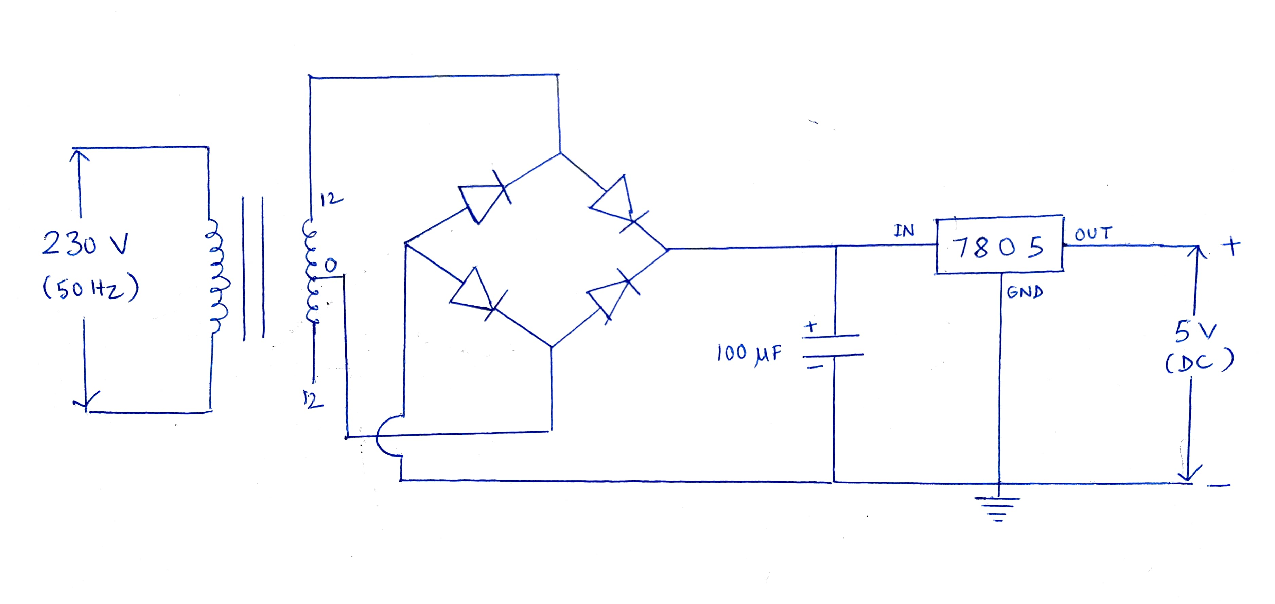
\includegraphics[width=\columnwidth]{figs/circuit}
    \caption{Schematic diagram of the circuit.}
    \label{fig:ckt}
\end{figure}

\section{Working}

\subsection{Step-down Transformer}
The step-down transformer was used to convert the 230 V AC mains voltage to 12 V AC\@. \\
The transformed voltage is given by
\[ v(t) = \SI[parse-numbers=false]{12\sqrt{2}\sin(100\pi t + \phi)}{\volt} \]
\begin{figure}[!htb]
    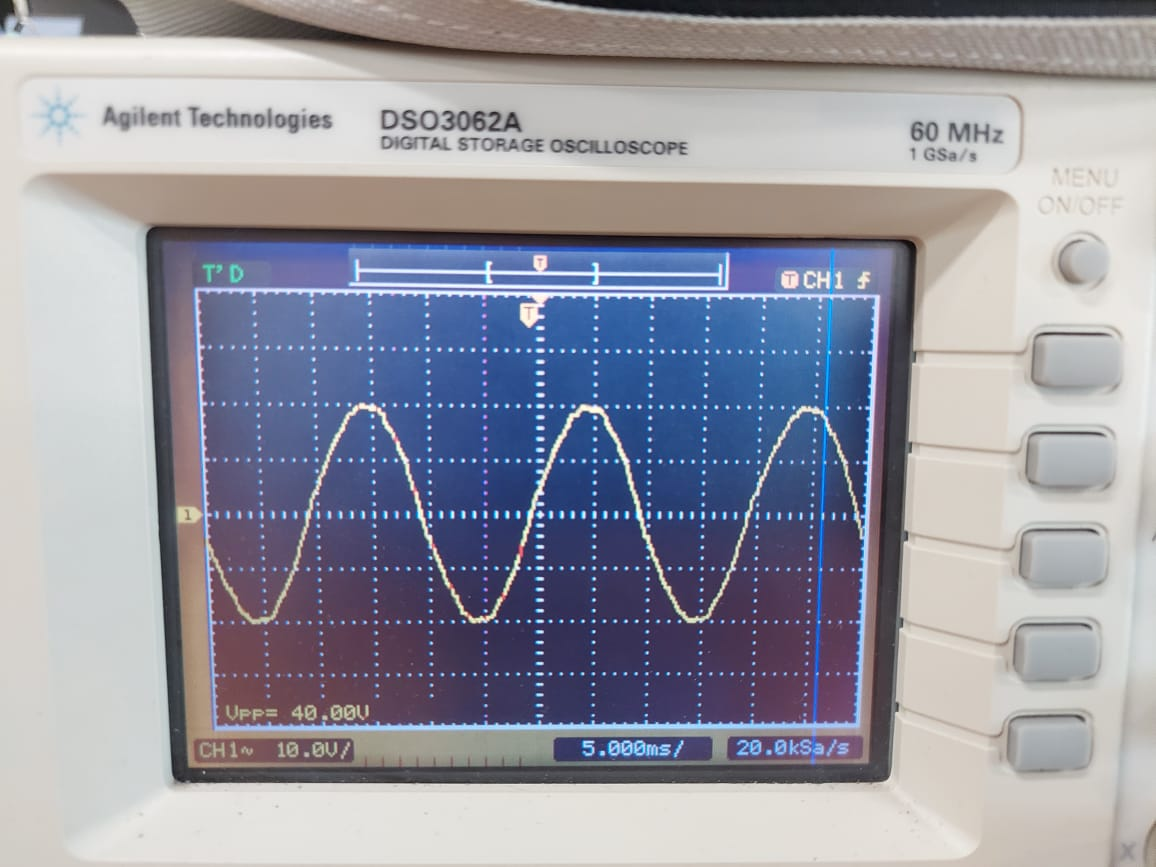
\includegraphics[width=\columnwidth]{figs/transformer}
    \caption{Transformer Readings}
    \label{fig:transformer}
\end{figure}

\subsection{Full-wave Bridge Rectifier}
The full-wave bridge rectifier was used to convert the AC voltage to DC\@.
\[ v(t) = \SI[parse-numbers=false]{12\sqrt{2} \abs{\sin(100\pi t + \phi)}}{\volt} \]


\subsection{Capacitor}
The capacitor is used as a low-pass filter to choose only the zero frequency component
converting the signal into a pure DC voltage \( \SI[parse-numbers=false]{12\sqrt{2}}{\volt} \).
\begin{figure}[!htb]
    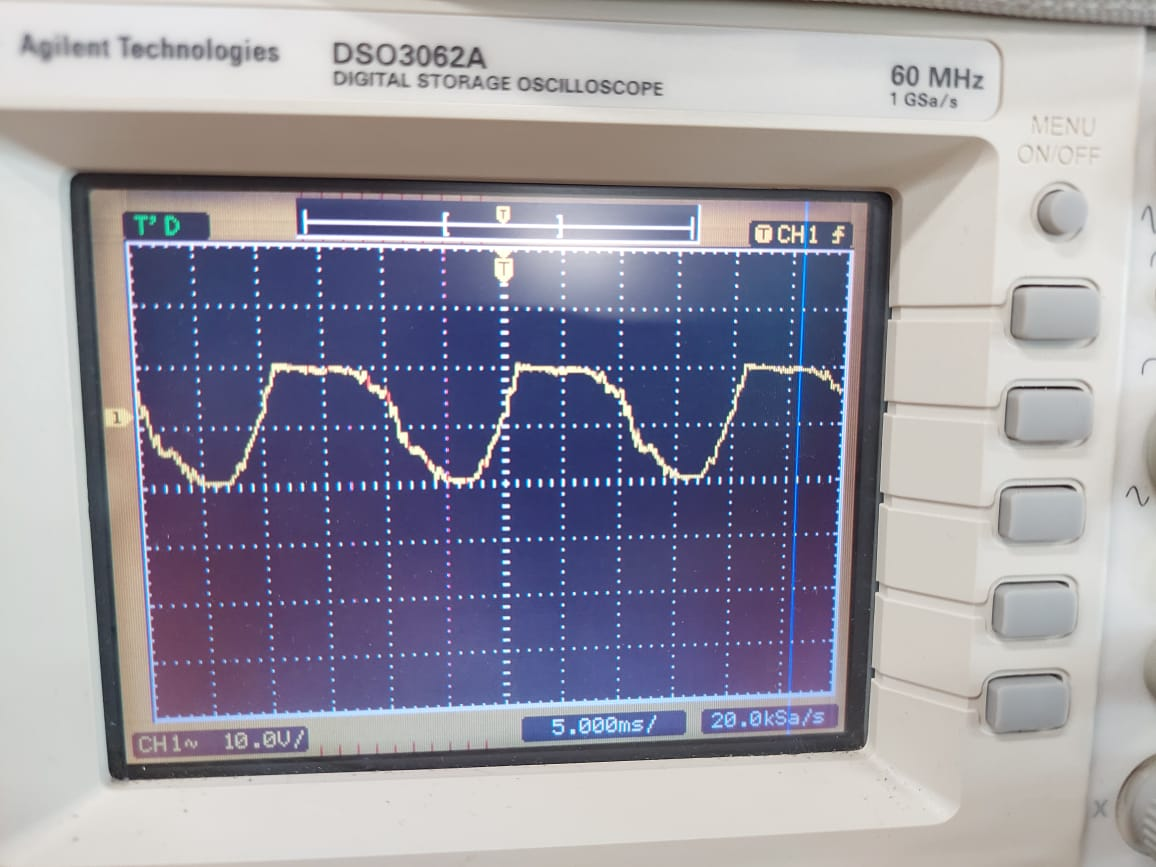
\includegraphics[width=\columnwidth]{figs/half-rectified}
    \caption{Half Wave Rectified Voltage}
    \label{fig:half-rectified}
\end{figure}


\subsection{Regulator}
The regulator is used to convert the DC voltage to a fixed voltage of \( \SI{5}{\volt} \).
\begin{figure}[!htb]
    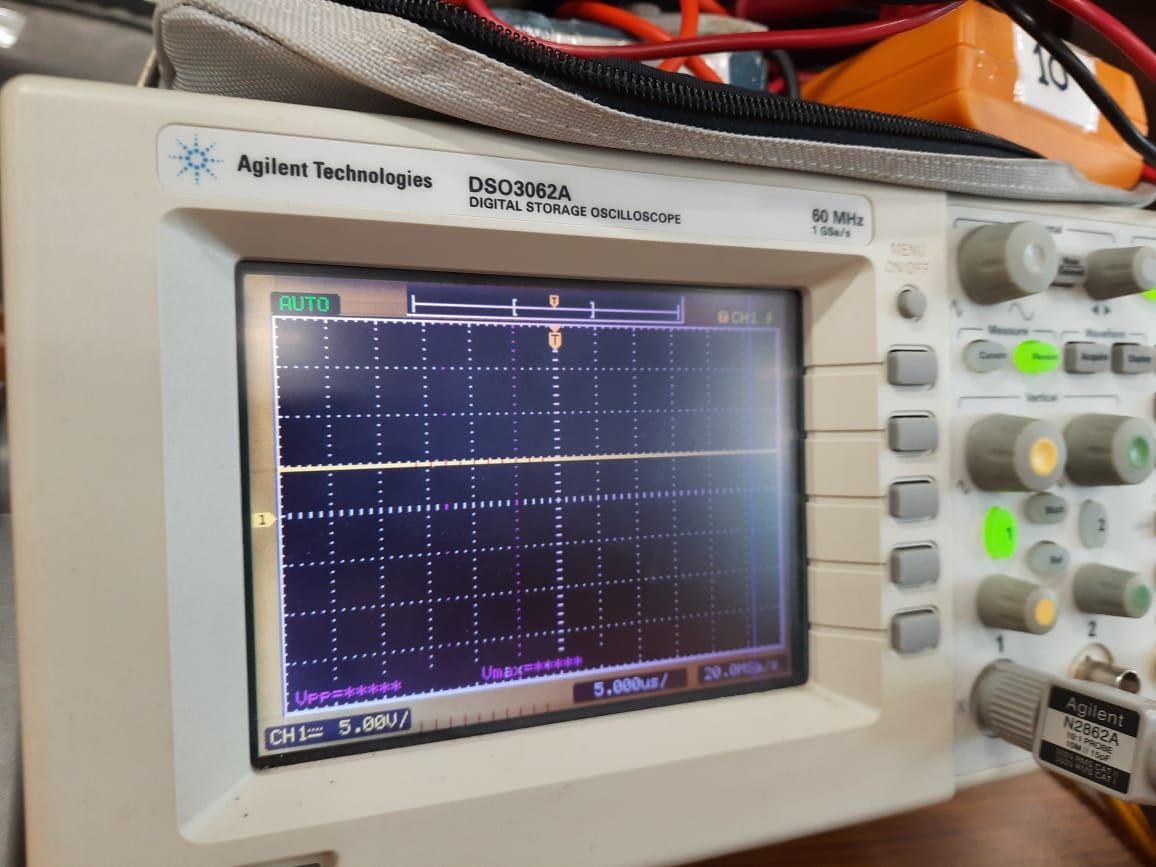
\includegraphics[width=\columnwidth]{figs/final}
    \caption{Fully Rectified Voltage}
    \label{fig:rectified}
\end{figure}

\section{Observations}
\begin{enumerate}
    \item Peak voltage after transformer and rectifier stage, 
        \( V_p = \SI[parse-numbers=false]{18}{\V} \).
    \item DC component after filter stage, 
        \( V_{DC} = \SI[parse-numbers=false]{18}{\V} \).
    \item DC component after regulator stage, $V_{DC}' = \SI{5}{\V}$.
\end{enumerate}

\section{Result}
Once the circuit is assembled and soldered and the output voltage is measured
to be \( \SI{5}{\volt} \) DC, the circuit is ready to be used. \\
Using a USB cable, the circuit can be used to charge a mobile phone or any other device.
An image of the circuit being used to charge a mobile phone is shown in Fig.~\ref{fig:phone}.

\begin{figure}[!htb]
    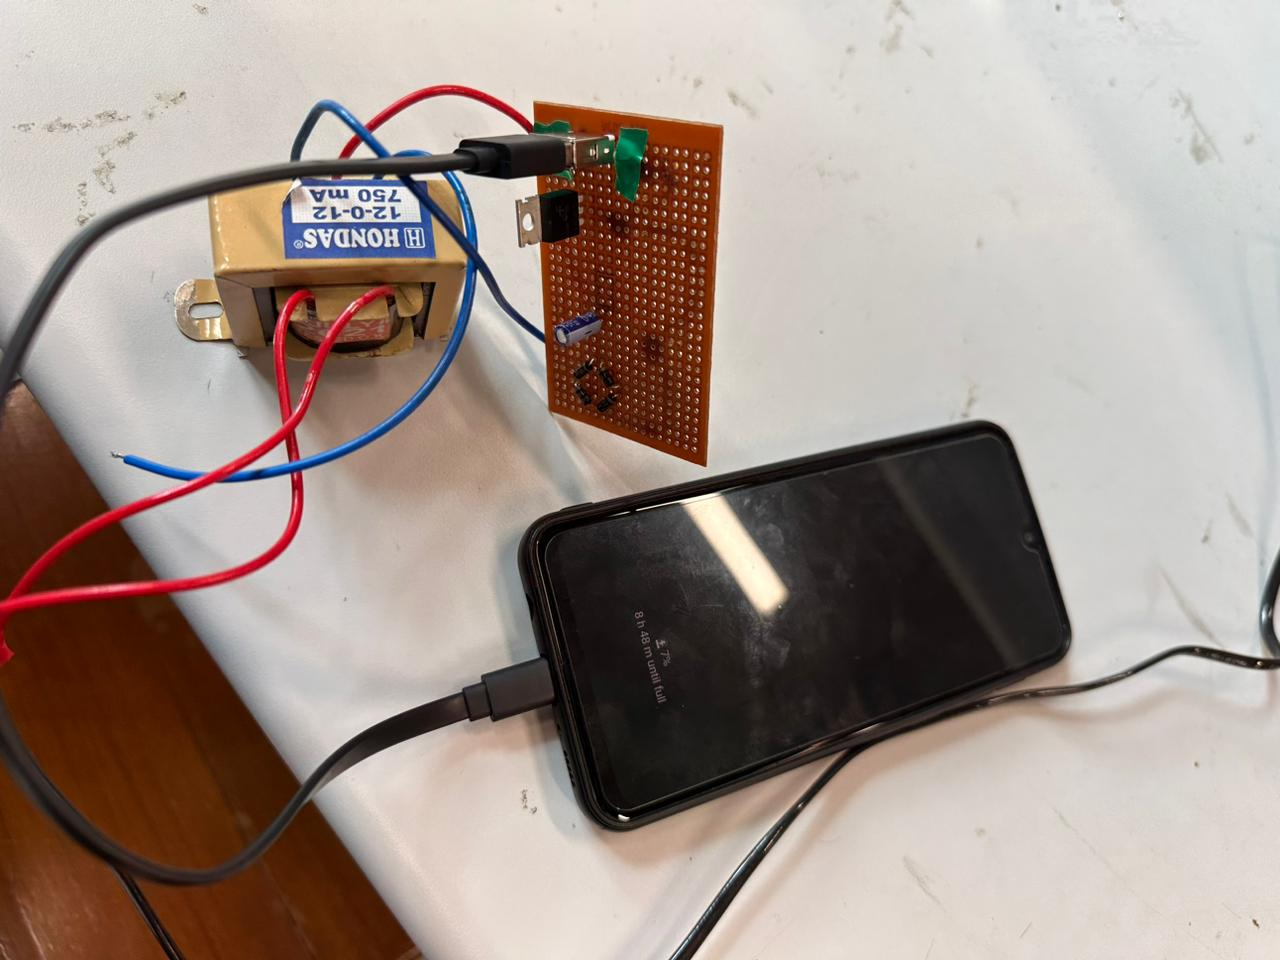
\includegraphics[keepaspectratio=true,width=\columnwidth]{figs/phone}
    \caption{Mobile Charging}
    \label{fig:phone}
\end{figure}


\end{document}